\documentclass{article}
\usepackage{blindtext}
\usepackage{tikz}
\usepackage[paperheight=295pt,paperwidth=794pt,margin=0pt]{geometry}
%,showframe
\usepackage{tikz}
\usepackage{tikz,fullpage}
\usetikzlibrary{arrows,%
                petri,%
                topaths}%
\usepackage{tkz-berge}
\usepackage[position=top]{subfig}
\usepackage{pgfplots}
\pgfplotsset{compat=1.12}

\title{\Huge{SOCIAL SCIENCE HACKATHON}}
\author{Room 35.3.xx}
\date{\emph{X. January 2018}}

\pagenumbering{gobble}

\begin{document}
\thispagestyle{empty}
\begin{minipage}[t][0pt]{\textwidth}
\maketitle
%\noindent\makebox[\linewidth]{\rule{\paperwidth}{0.4pt}}
\center{\textit{\Large{Some encouraging text, making it seem like fun to spend an entire day writing code.}}}

\vspace{-7cm}
\hspace{12cm}
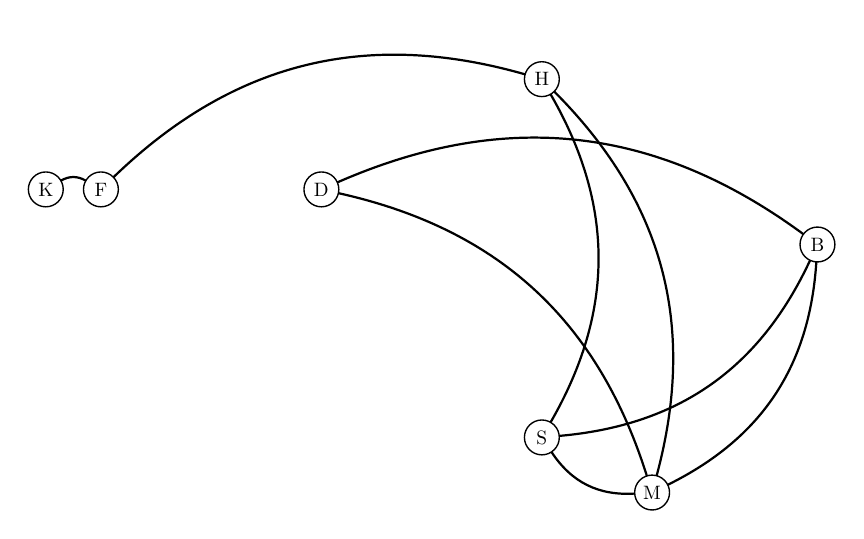
\begin{tikzpicture}[scale=0.7,transform shape]
  \Vertex[x=-6,y=6]{K}
  \Vertex[x=-5,y=6]{F}
  \Vertex[x=-1,y=6]{D}
  \Vertex[x=3,y=8]{H}
  \Vertex[x=8,y=5]{B}
%  \Vertex[x=9,y=2]{N}
  \Vertex[x=5,y=0.5]{M}
  \Vertex[x=3,y=1.5]{S}
  \tikzstyle{LabelStyle}=[fill=white,sloped]
  \tikzstyle{EdgeStyle}=[bend left]
  \Edge[](K)(F)
  \Edge[](H)(S)
  \Edge[](H)(M)
  \Edge[](D)(B)
  \Edge[](D)(M)
  \Edge[](B)(M)
%  \Edge[](H)(N)
  \Edge[](F)(H)
  \tikzstyle{EdgeStyle}=[bend right]
  \Edge[](S)(B)
%  \Edge[](S)(N)
  \Edge[](S)(M)
\end{tikzpicture}
%
% \vspace{-7cm}
% \hspace{-24cm}
% \begin{tikzpicture}[scale = 1.5]
%   \pgfplotsset{ticks=none}
%  \begin{axis}[axis line style={draw=none},
%       tick style={draw=none}]
% % xtick=data,
%  xticklabels = {draw=none}
% % {/pgf/number format/1000 sep=,rotate=60,anchor=east,font=\scriptsize},
% % ylabel=,
% % ]
% \addplot
% coordinates {(1000,98.37390698103358)
% (1001,100.96441372901103)
% (1002,98.28903819562608)
% (1003,101.3584712513718)
% (1004,102.17249882217783)
% (1005,101.36103716362516)
% (1006,102.38585375437282)
% (1007,95.21601797761495)
% (1008,97.2684533193606)
% (1009,101.42390386235117)
% (1010,100.9567667934013)
% (1011,101.96323243416526)
% (1012,99.24362080120177)
% (1013,101.92586923776655)
% (1014,97.73973262019145)
% (1015,113.49783523714402)
% (1016,101.17151360171636)
% (1017,98.94813092791472)
% (1018,99.83677117194605)
% (1019,102.46236310144461)
% (1020,99.23779488464817)
% (1021,101.39943376084052)
% (1022,102.27801935944802)
% (1023,103.4721413180812)
% (1024,98.83898737629247)
% (1025,104.51615638200617)
% (1026,103.5468703639049)
% (1027,104.1803000399682)
% (1028,106.10751762026958)
% (1029,103.96827259518689)
% (1030,101.41227858587958)
% (1031,106.84273586484464)
% (1032,103.46875571383498)
% (1033,101.3133323944154)
% (1034,106.36608923564054)
% (1035,98.31746468063164)
% (1036,102.68221774298715)
% (1037,108.29339049549434)
% (1038,105.75376981314345)
% (1039,102.08986619098556)
% (1040,107.26962814064703)
% (1041,103.9672631215834)
% (1042,99.11564787836248)
% (1043,98.17062843423477)
% (1044,104.99991052890131)
% (1045,103.47485338574744)
% (1046,106.94660385561488)
% (1047,108.0010452420808)
% (1048,104.54374407057782)
% (1049,104.13759344315024)
% (1050,110.51875953990572)
% (1051,110.94448076775404)
% (1052,105.21016717029201)
% (1053,104.45290879647689)
% (1054,109.34784879271342)
% (1055,110.51015116166883)
% (1056,107.20344355424777)
% (1057,104.16035384062963)
% (1058,106.04027707987001)
% (1059,103.17770845831153)
% (1060,106.08413649363162)
% (1061,107.86054467391162)
% (1062,104.02575383999483)
% (1063,104.28646654029608)
% (1064,109.44109375393917)
% (1065,106.30414498121196)
% (1066,104.44688317416913)
% (1067,104.77015137825725)
% (1068,110.70543842235456)
% (1069,107.25788398365658)
% (1070,105.26216970110472)
% (1071,107.8962317509465)
% (1072,106.38183660518256)
% (1073,99.08601046549424)
% (1074,108.88700084684051)
% (1075,107.53283807641215)
% (1076,110.81798127897032)
% (1077,99.94438137722565)
% (1078,103.51085087312667)
% (1079,103.38394125234768)
% (1080,107.3918531518424)
% (1081,107.44077706380008)
% (1082,106.5668319914415)
% (1083,114.10816455932721)
% (1084,104.52384346565329)
% (1085,111.18523552185837)
% (1086,106.9502434704995)
% (1087,107.19170686973371)
% (1088,108.94706609940378)
% (1089,105.71540325130567)
% (1090,106.84886501277353)
% (1091,106.19792224959055)
% (1092,108.6387809188954)
% (1093,107.83048934450908)
% (1094,111.63250495247891)
% (1095,108.18041469850466)
% (1096,108.64992128907286)
% (1097,106.91089762832162)
% (1098,106.82928930546278)
% (1099,105.61528211760118)};
%  \end{axis}
% \end{tikzpicture}

\end{minipage}

\end{document}
